On dispose d'un dé cubique non truqué dont les faces opposées sont identiques : deux faces numérotées 0, deux faces numérotées 1 et deux faces numérotées $2 .$

\begin{enumerate}
  \item On effectue deux lancers et on lit, à chaque lancer, le chiffre inscrit sur la face supérieure. Les deux lancers permettent d'obtenir un nombre décimal : le résultat du premier lancer donne le chiffre des unités et celui du second lancer le chiffre des dixièmes.
  
  \begin{enumerate}
  	\item Donner la liste de tous les nombres que l'on peut obtenir.
  	\item Justifier que la probabilité d'obtenir 1,2 est égale à $1 / 9$.
  	\item Quelle est la probabilité d'obtenir un nombre strictement inférieur à 1 ?
  	\item Quelle est la probabilité d'obtenir un nombre entier ?
  	\item Quelle est la probabilité d'obtenir un nombre décimal ?
  \end{enumerate}

  \begin{minipage}[t]{.7\linewidth}
  \item 
  
  Le tapis représenté ci-contre est constitué de 36 carrés de côté $10 \mathrm{~cm}$. Ces carrés définissent trois zones $Z_1$, $Z_2$ et $Z_3$ repérées par des couleurs différentes. Avec le même dé que précédemment, on effectue un lancer sur ce tapis et on regarde la face supérieure. Si le dé tombe à cheval sur deux zones, on le relance. On admet que la probabilité que le dé tombe dans une zone est proportionnelle à l'aire de la zone.	
	
	\begin{enumerate}
	\item Quelle est la probabilité que le dé tombe dans la zone $Z_{2}$ ?
	\item Quelle est la probabilité que le dé tombe en zone $Z_{2}$ et donne le nombre 1 ?
	\item Quelle est la probabilité que le dé tombe en zone $Z_{2}$ et donne un nombre pair ?
\end{enumerate}

  \end{minipage}
  \begin{minipage}[t]{.3\linewidth}
    \vspace{0cm}
    \centering
  	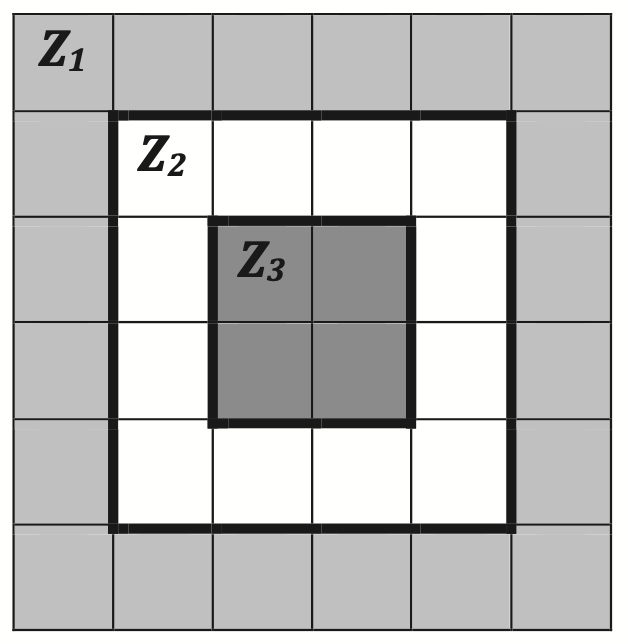
\includegraphics[width=.9\linewidth]{2022-g1-ex2-img1.png}
  \end{minipage}
  
\end{enumerate}